\documentclass[12pt, a4paper]{article}
\usepackage{ctex}
\usepackage{amsmath,amscd,amsbsy,amssymb,latexsym,url,bm,amsthm}
\usepackage{caption}
\usepackage{epsfig,graphicx,subfigure}
\usepackage{enumitem,balance}
\usepackage{wrapfig}
\usepackage{listings}
\usepackage{mathrsfs,euscript}
\usepackage[usenames]{xcolor}
\usepackage{hyperref}
\usepackage[vlined,ruled,linesnumbered]{algorithm2e}
\hypersetup{colorlinks=true,linkcolor=black}

\captionsetup[figure]{
	labelfont = {bf},
	labelformat = {default},
	labelsep = period,
	name = {Fig.}
}

\captionsetup[table]{
	labelfont = {bf},
	labelformat = {default},
	labelsep = period,
	name = {Tab.}
}

\newtheorem{theorem}{Theorem}
\newtheorem{lemma}[theorem]{Lemma}
\newtheorem{proposition}[theorem]{Proposition}
\newtheorem{corollary}[theorem]{Corollary}
\newtheorem{exercise}{Exercise}
\newtheorem*{solution}{Solution}
\newtheorem{definition}{Definition}
\theoremstyle{definition}
\lstset{
	keywordstyle = \color{blue!70}\bfseries, 
	basicstyle = \ttfamily, 
	commentstyle = \ttfamily,
	showstringspaces = false,
	frame = shadowbox,
	rulesepcolor = \color{red!20!green!20!blue!20},
}

\renewcommand{\thefootnote}{\fnsymbol{footnote}}

\newcommand{\postscript}[2]{
	\setlength{\epsfxsize}{#2\hsize}
  	\centerline{\epsfbox{#1}}
}

\renewcommand{\baselinestretch}{1.0}

\setlength{\oddsidemargin}{-0.35in}
\setlength{\evensidemargin}{-0.35in}
\setlength{\topmargin}{-0.3in}
\setlength{\headheight}{0in}
\setlength{\headsep}{0in}
\setlength{\textheight}{10.2in}
\setlength{\textwidth}{7in}
\makeatletter 
\renewenvironment{proof}[1][Proof] {\par\pushQED{\qed}\normalfont\topsep6\p@\@plus6\p@\relax\trivlist\item[\hskip\labelsep\bfseries#1\@addpunct{.}]\ignorespaces}{\popQED\endtrivlist\@endpefalse} \makeatother
\makeatletter
\renewenvironment{solution}[1][Solution] {\par\pushQED{\qed}\normalfont\topsep6\p@\@plus6\p@\relax\trivlist\item[\hskip\labelsep\bfseries#1\@addpunct{.}]\ignorespaces}{\popQED\endtrivlist\@endpefalse} \makeatother

\begin{document}
\noindent

%========================================================================
\noindent\framebox[\linewidth]{\shortstack[c]{
\Large{\textbf{Lab \#4: Table Reconstruction}}\vspace{1mm}\\
EE447 Mobile Network, Luoyi Fu, Spring 2021\\
\textbf{Due}: \textit{Sunday, June 13th}}}
\begin{center}

Name: Hongjie Fang  \quad Student ID:518030910150 \quad Email: \href{mailto:galaxies@sjtu.edu.cn}{galaxies@sjtu.edu.cn}
\end{center}

\section{Purpose and Objective}\label{section1}

Nowadays, PDF documents have become the mainstream document format because of its unique cross-platform convenience advantage. PDF documents contain a large amount of valuable data information, and the table is one of the important carriers of these data. However, the structure of PDF documents is complex, and it is difficult for us to obtain accurate table information directly from the document format. Therefore, for PDF tables, we need to reconstruct the structure of the table, so as to achieve the extraction of the table.

PDF documents are often used in academic paper writing, therefore in this lab, we mainly focus on the table reconstruction in academic papers. The table reconstruction may help a lot in information extraction from PDFs, especially structured data extraction. 

This Lab focuses on the table line reconstruction for the tables without frame lines. In this Lab, we are required to use python to complete table line drawing of a specific table without frame lines and show the results. After that, there are three questions:

\begin{enumerate}
	\item How to automatically locate the tables in a PDF?
	\item What do you think is the most difficult step to extract the table from the PDF? Why?
	\item \textbf{(Bonus)} How to accurately identify the header of the table, and use natural language processing (NLP) or other methods to understand the information in the table, and then extract the entities and relationships from table to construct a specific knowledge graph?
\end{enumerate}

\section{Frameline-drawing Algorithm}\label{section2}
In this section, we will explain the algorithm of completing table frameline drawing in given code.

\begin{itemize}
	\item We first convert the image to gray-scale image, which will make things easier since we do not need to worry about the color of the word in the table. Then, we extract the edges of the table, which is used to detect the partial-drawing lines in the table.
	\item After that, we erase the partial-drawing lines from the table, and detect the boundary of the table (up-left point and down-right point). Then, we can remove the bounding lines of the table. Then, we erode the image slightly and perform binaryzation for convenience.
	\item Next, we detect the horizontal lines, if we have sacnned a all-white line, then it may be the boundary between two lines in the table. Therefore we can record it in the list. If we find several continuous ``potential boundary'', we can combine them into one using the average value of the $y$ coordinates.
	\item Similarly, we transpose the image and then perform the same operation again to detect the vertical lines.
	\item Finally, we combine the horizontal lines and vertical lines, and draw these lines in the picture.
\end{itemize}

We implement the algorithm based on the given code in python. Fig. \ref{fig1}, Fig. \ref{fig2}, Fig. \ref{fig3}, Fig. \ref{fig4} and Fig. \ref{fig5} are the results.

\begin{figure}[htbp]
	\centering
		\begin{minipage}[t]{0.9\linewidth}
		\centering
		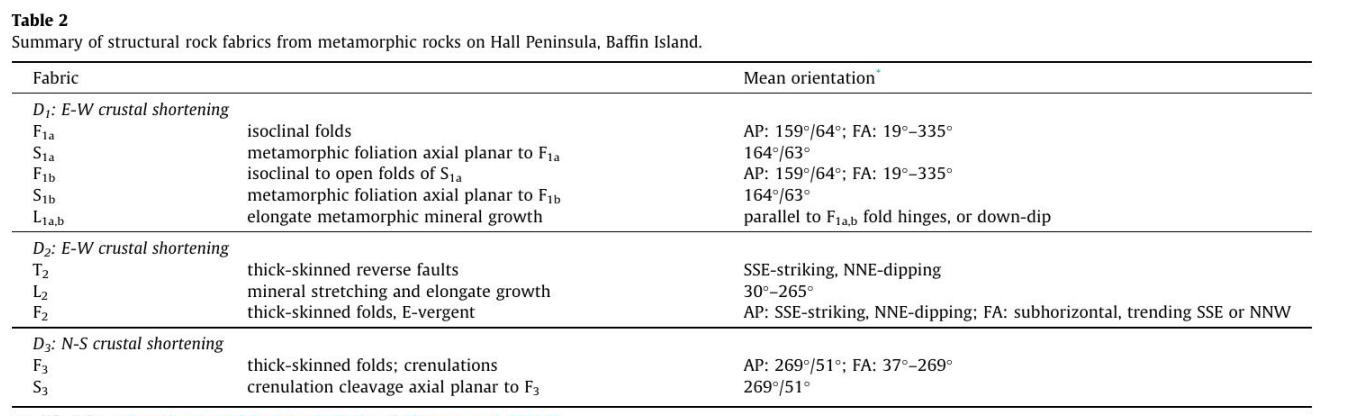
\includegraphics[width=\linewidth]{1.png}
		\end{minipage}
		\linebreak 
		\begin{minipage}[t]{0.9\linewidth}
		\centering
		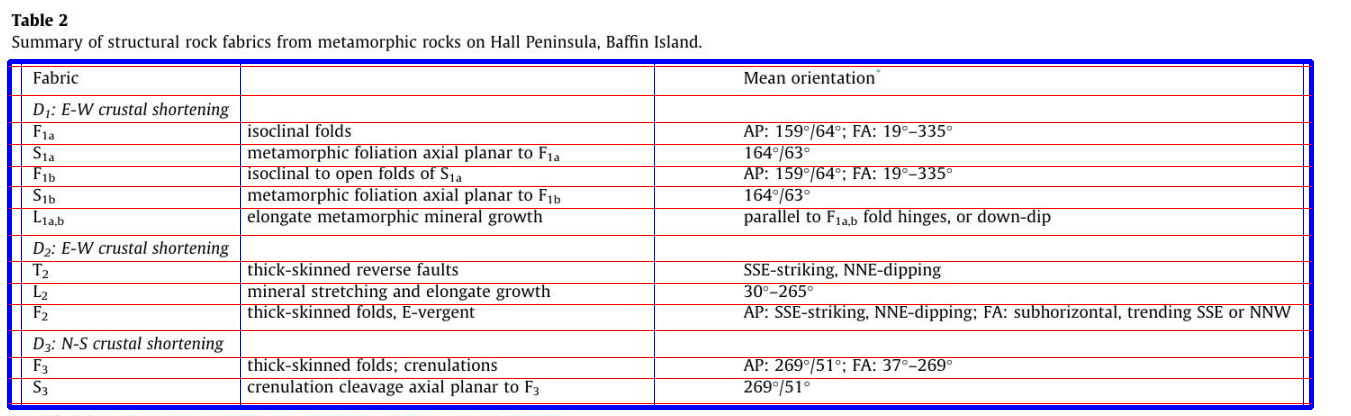
\includegraphics[width=\linewidth]{reconstructed_1.png}
		\end{minipage}
	\caption{The original table and the reconstructed table (1)}
	\label{fig1}
\end{figure}
\begin{figure}[htbp]
	\centering
		\begin{minipage}[t]{0.9\linewidth}
		\centering
		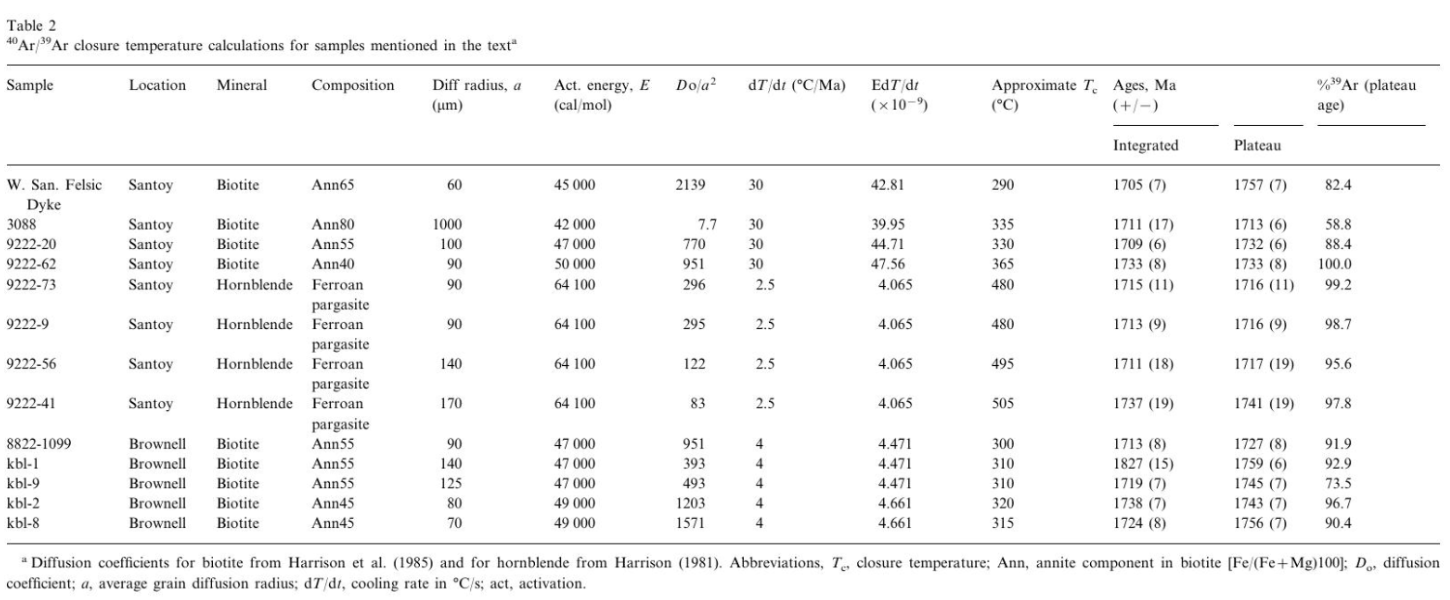
\includegraphics[width=\linewidth]{2.png}
		\end{minipage}
		\linebreak 
		\begin{minipage}[t]{0.9\linewidth}
		\centering
		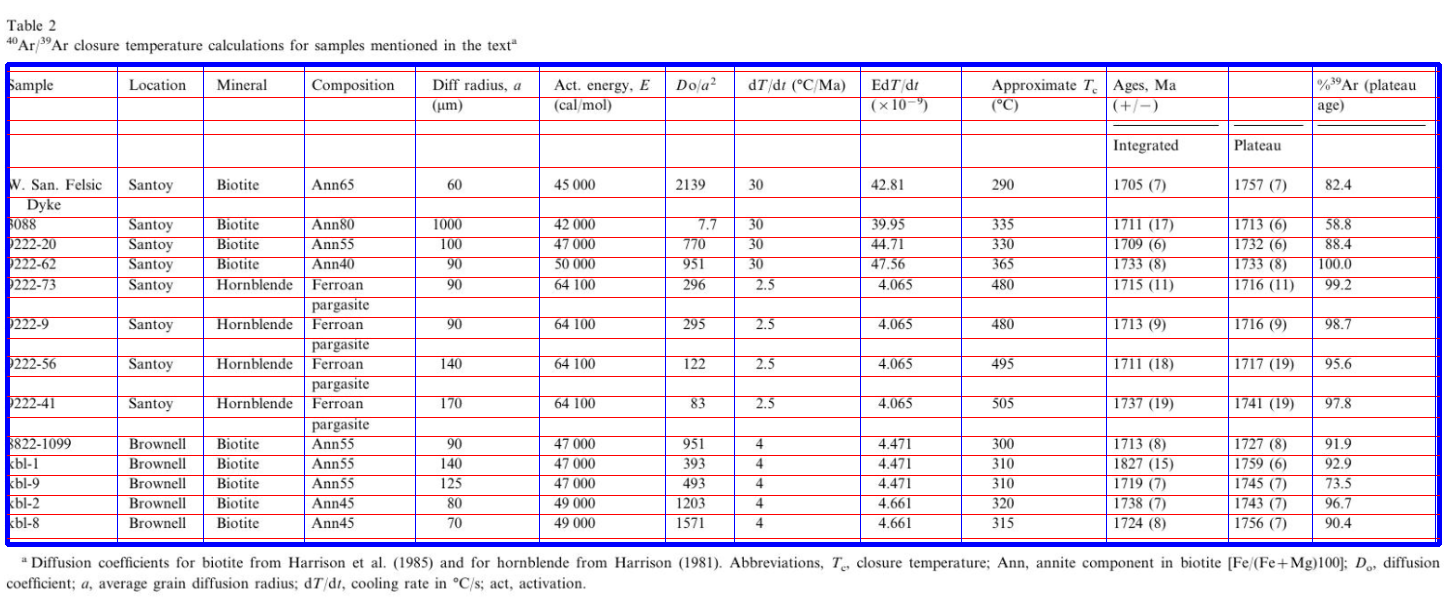
\includegraphics[width=\linewidth]{reconstructed_2.png}
		\end{minipage}
	\caption{The original table and the reconstructed table (2)}
	\label{fig2}
\end{figure}
\begin{figure}[htbp]
	\centering
		\begin{minipage}[t]{0.9\linewidth}
		\centering
		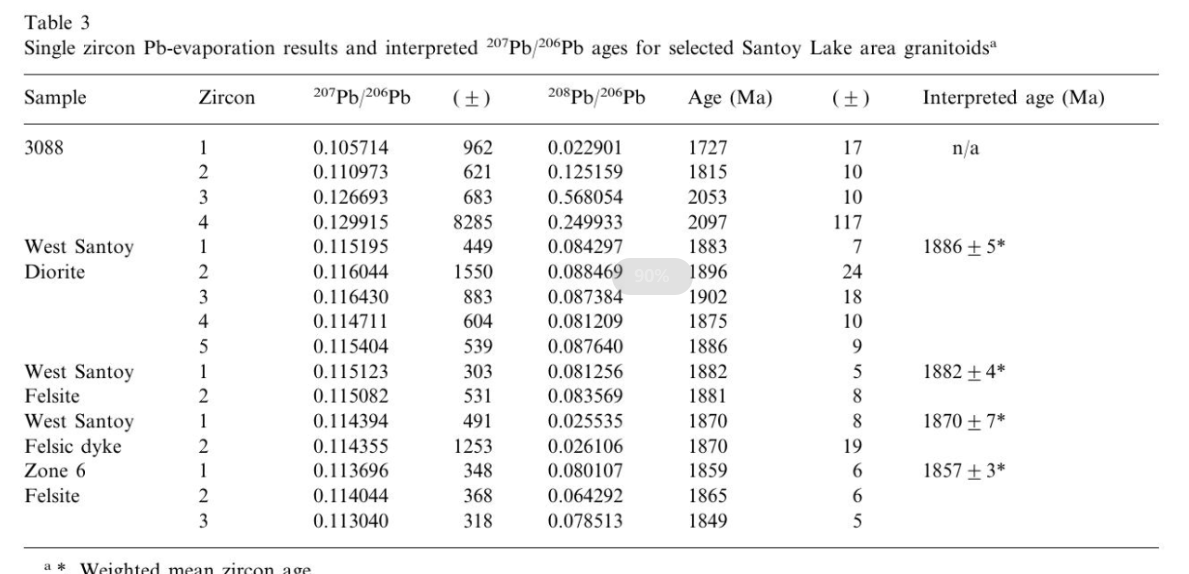
\includegraphics[width=\linewidth]{3.png}
		\end{minipage}
		\linebreak 
		\begin{minipage}[t]{0.9\linewidth}
		\centering
		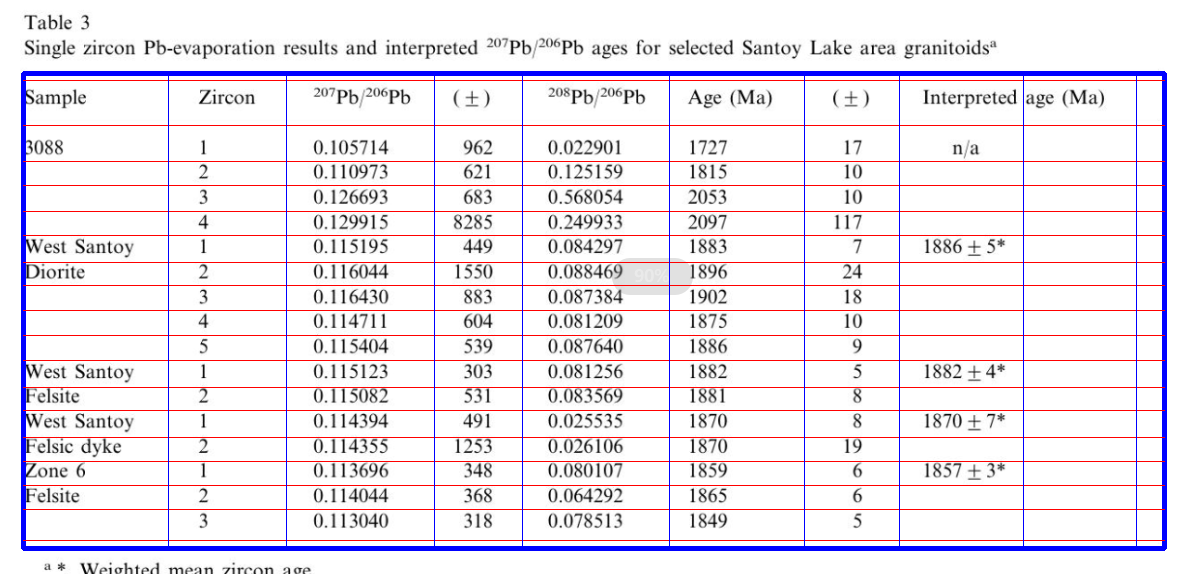
\includegraphics[width=\linewidth]{reconstructed_3.png}
		\end{minipage}
	\caption{The original table and the reconstructed table (3)}
	\label{fig3}
\end{figure}
\begin{figure}[htbp]
	\centering
		\begin{minipage}[t]{0.4\linewidth}
		\centering
		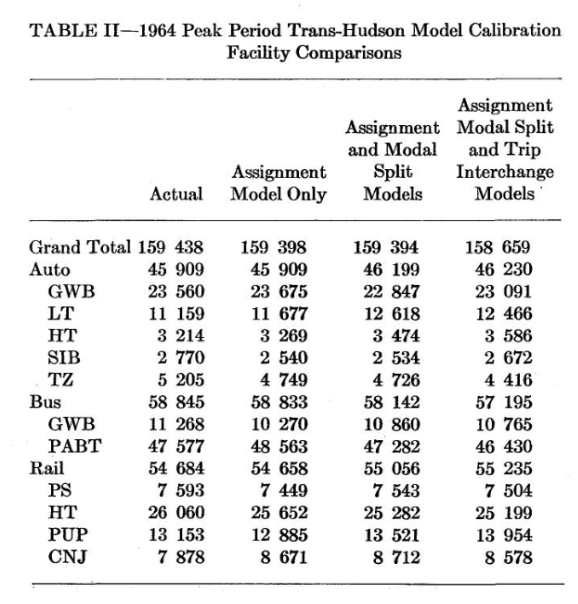
\includegraphics[width=\linewidth]{4.png}
		\end{minipage}
		\begin{minipage}[t]{0.4\linewidth}
		\centering
		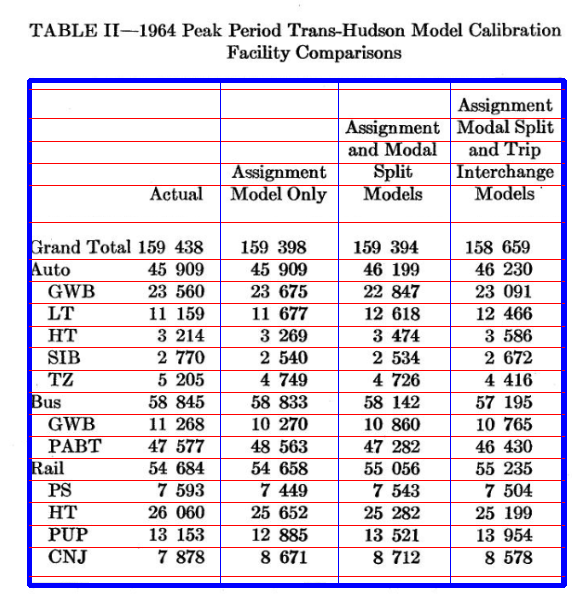
\includegraphics[width=\linewidth]{reconstructed_4.png}
		\end{minipage}
	\caption{The original table and the reconstructed table (4)}
	\label{fig4}
\end{figure}
\begin{figure}[htbp]
	\centering
		\begin{minipage}[t]{0.9\linewidth}
		\centering
		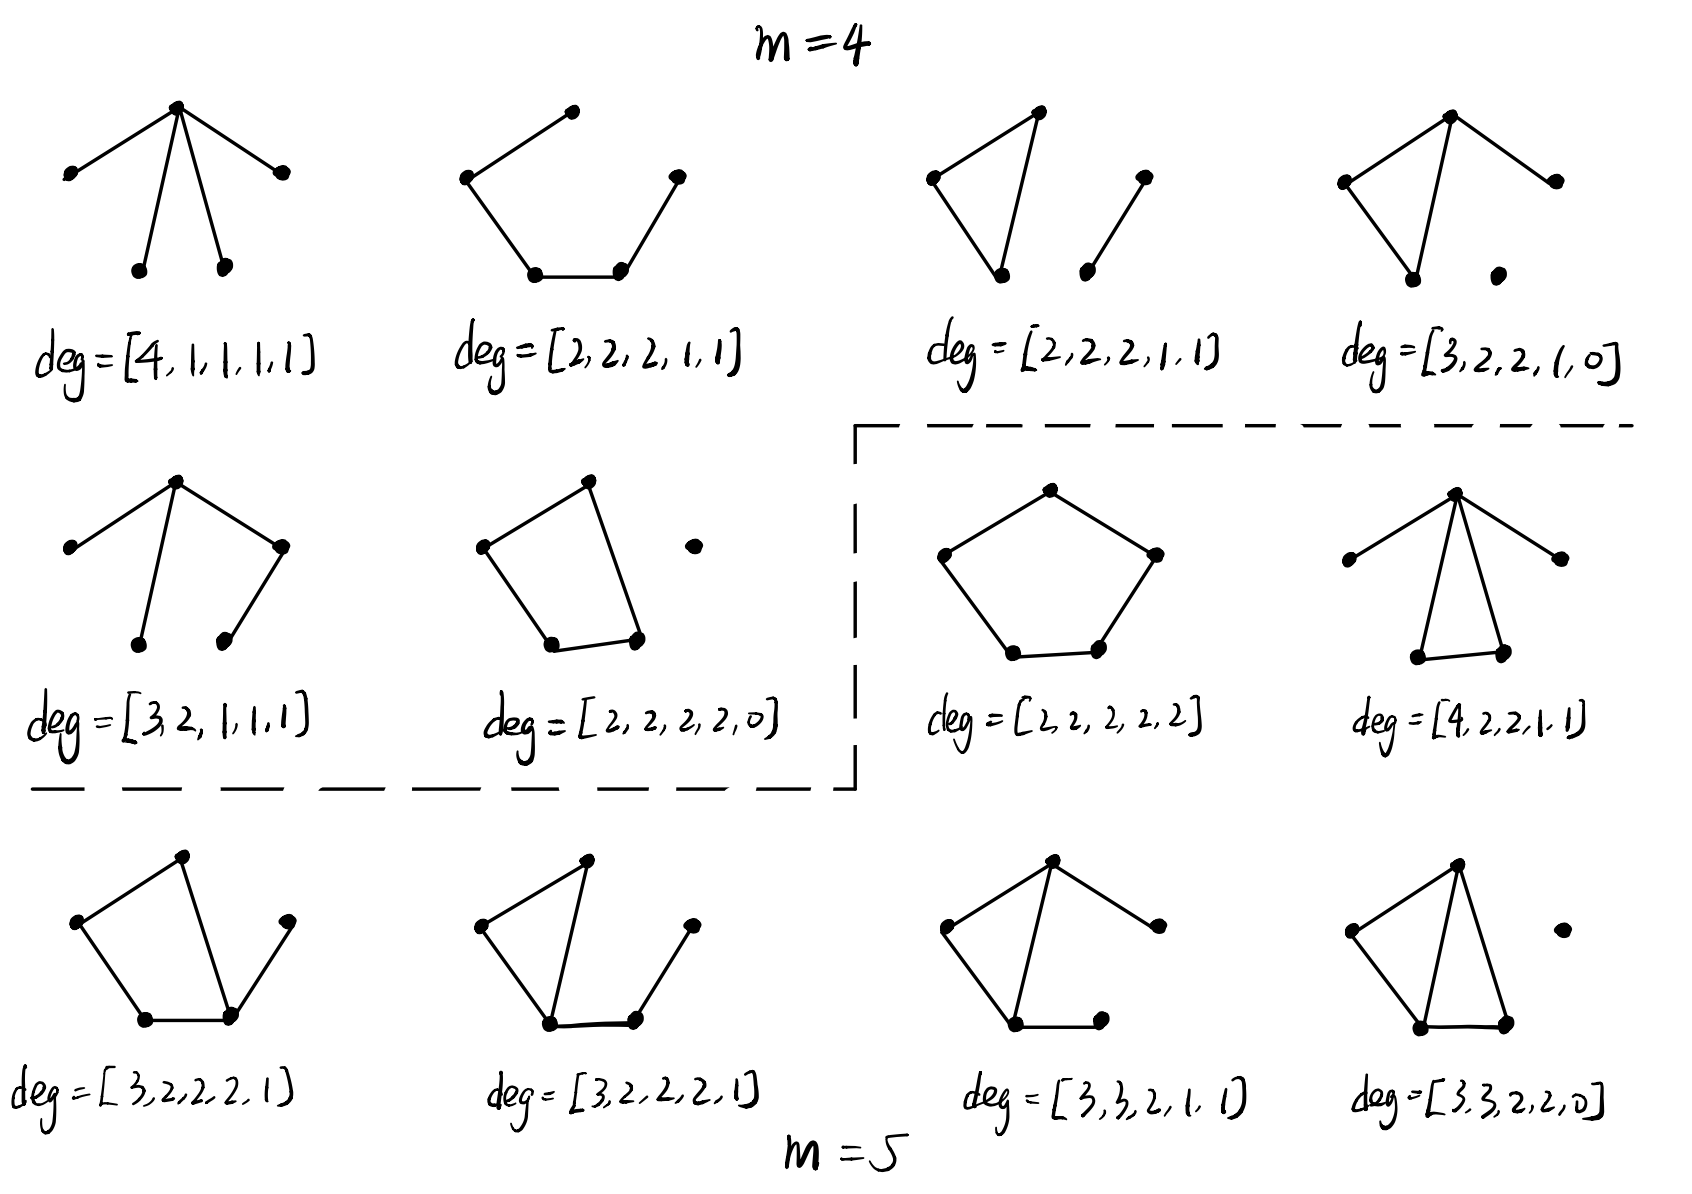
\includegraphics[width=\linewidth]{5.jpg}
		\end{minipage}
		\linebreak 
		\begin{minipage}[t]{0.9\linewidth}
		\centering
		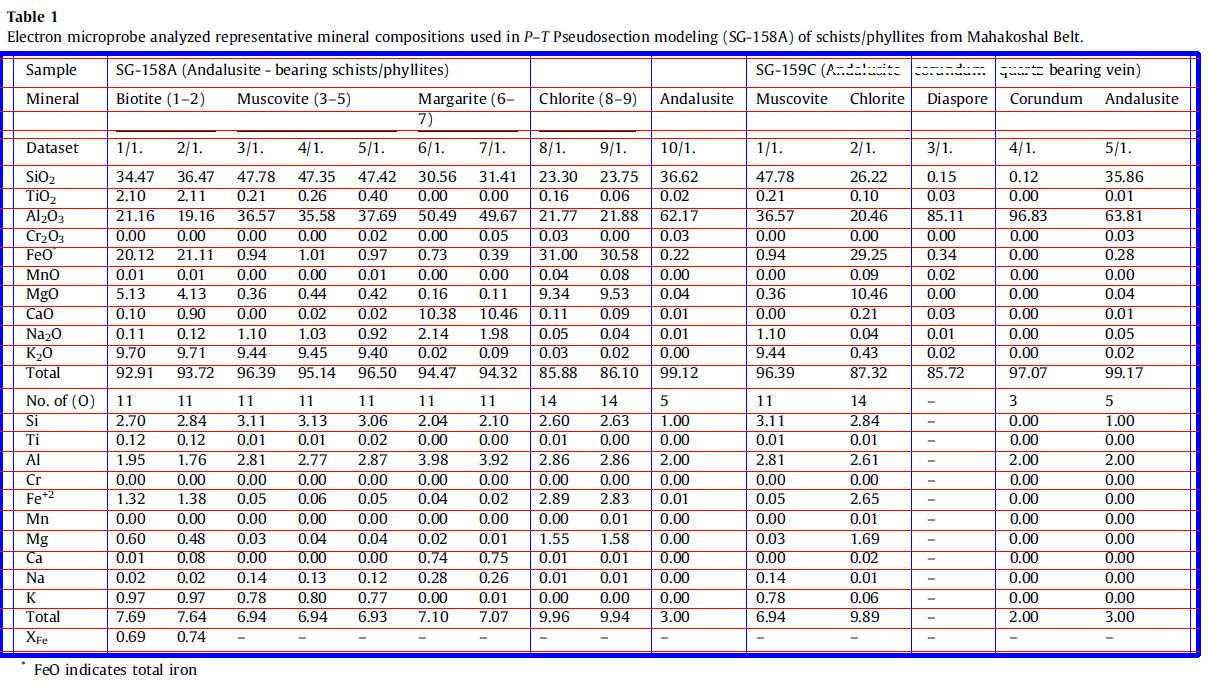
\includegraphics[width=\linewidth]{reconstructed_5.png}
		\end{minipage}
	\caption{The original table and the reconstructed table (5)}
	\label{fig5}
\end{figure}

\paragraph{Analyses} From results we can observe that, our algorithm can detect the table boundary accurately, which completes table reconstruction task.

\section{Extracting Tables from PDFs}
We use a open-source project pdftotree\footnotemark[1] to
get the hierarchical tree of context objects such as text blocks, figures, tables, etc. For tables, it will extract their bounding boxes. Therefore, we can use the bounding boxes to extract tables from PDF files. Here is the specific pipeline:
\begin{enumerate}
\item Use pdftotree\footnotemark[1] to get the hierarchical tree of the context objects.
\item Find table objects in the tree extracted in step 1, and get the bounding boxes of the tables from the extracted tree.
\item Extract tables according to the bounding boxes.
\end{enumerate}

Here is an example of the bounding boxes we extracted from a PDF paper\footnotemark[2].

\begin{figure}[htbp]
	\centering
	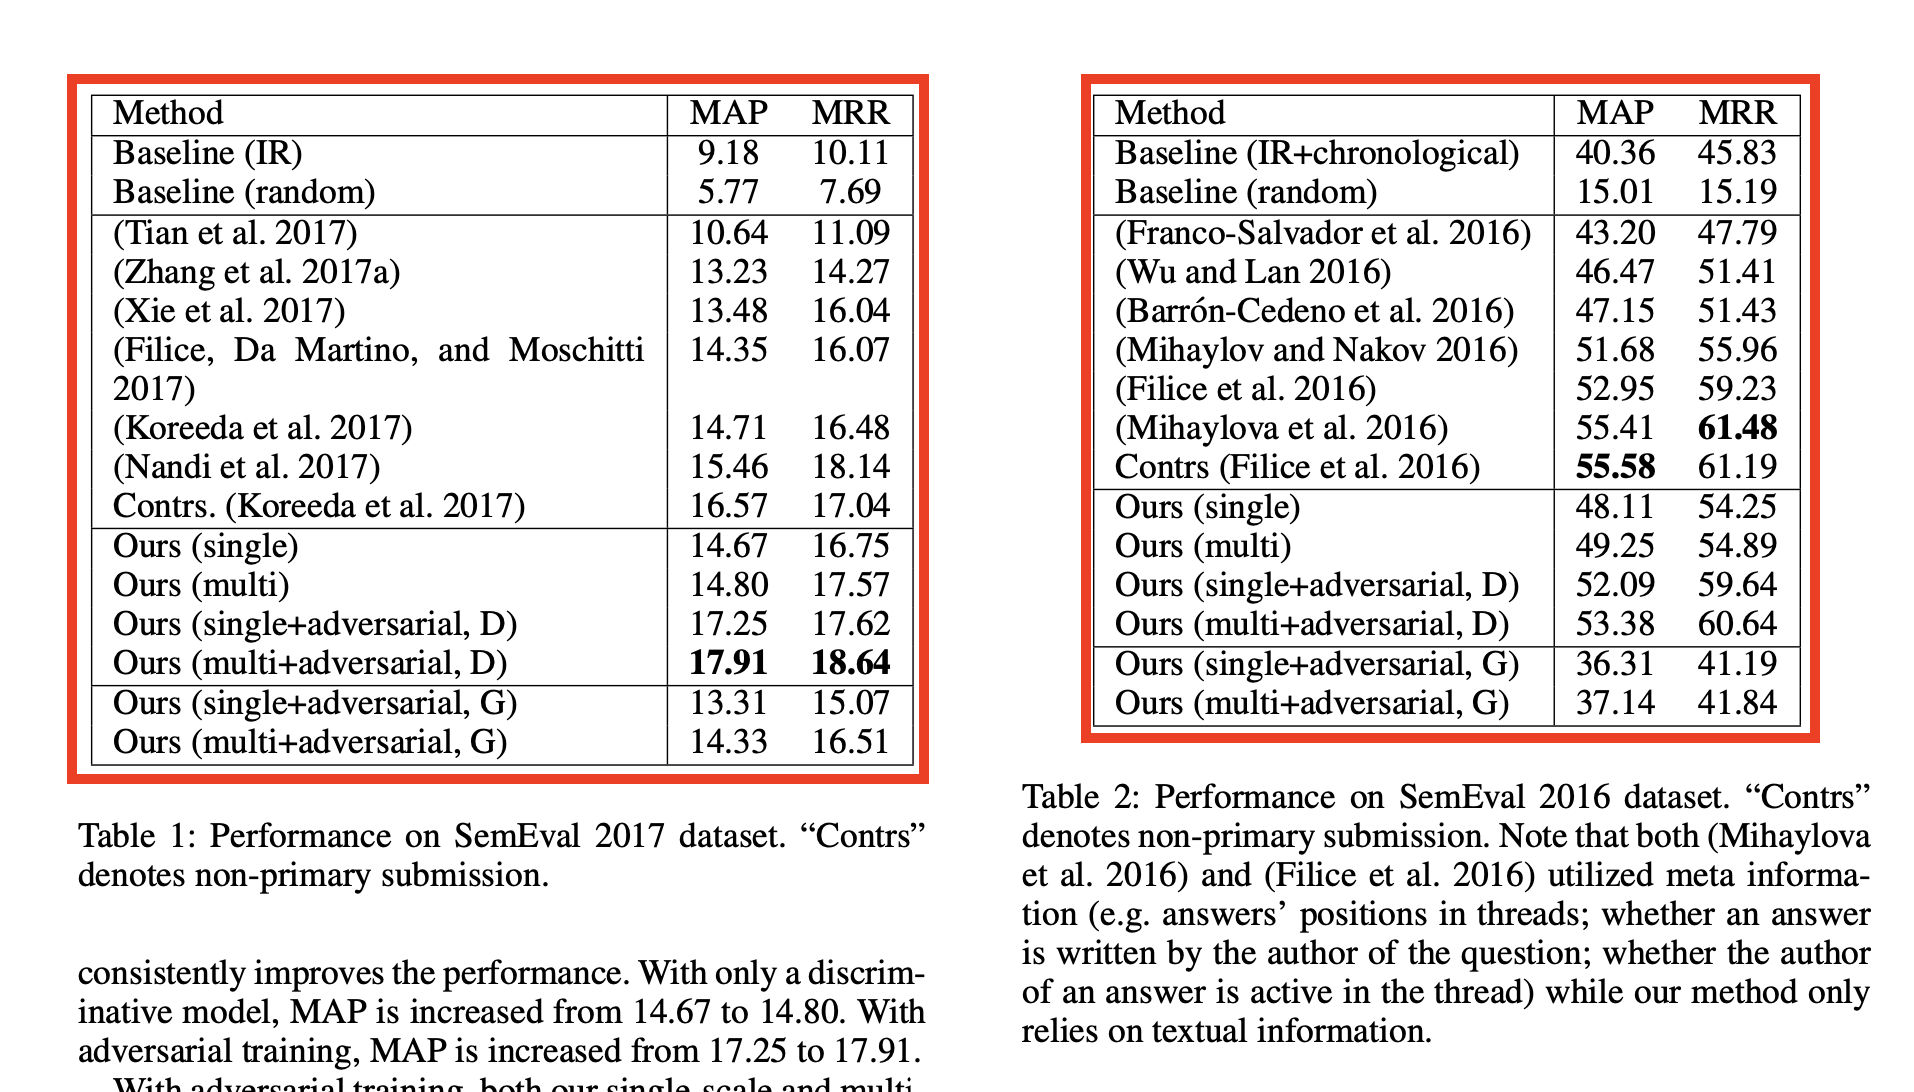
\includegraphics[width=0.9\linewidth]{table-bounding-boxes.png}
	\caption{The bounding boxes of the table, which is extracted using pdftotree}
	\label{fig6.5}
\end{figure}

Then, we can easily extract the images from the PDF file, and use the algorithms introduced in Section \ref{section2} to draw the framelines. The results are shown in Fig. \ref{fig6.8} in the next page. Therefore, we have successfully build a pipeline to extract tables from PDFs and reconstruct the framelines of the tables.


\begin{figure}[htbp]
	\centering
		\begin{minipage}[t]{0.4\linewidth}
		\centering
		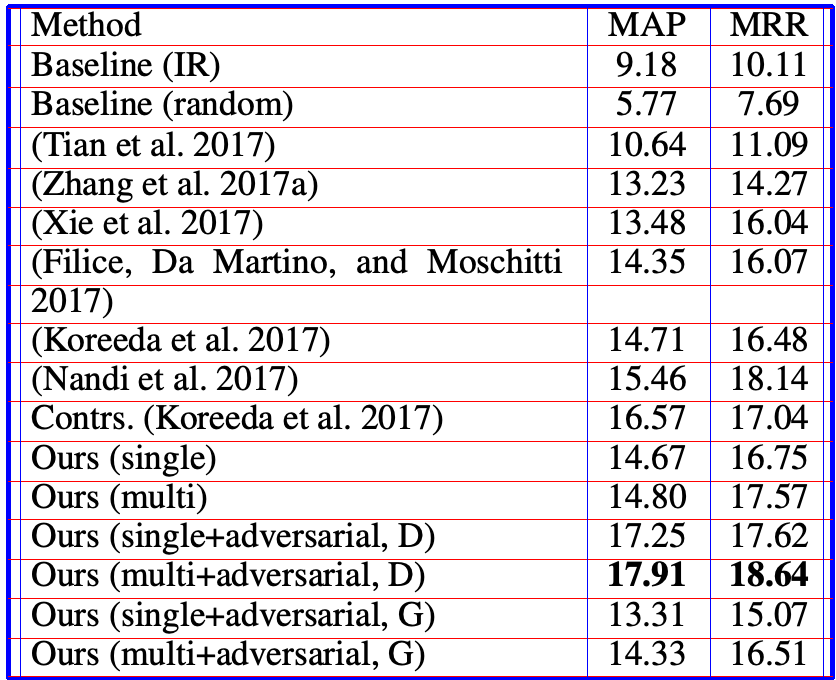
\includegraphics[width=\linewidth]{reconstructed_6.png}
		\end{minipage}
		\begin{minipage}[t]{0.4\linewidth}
		\centering
		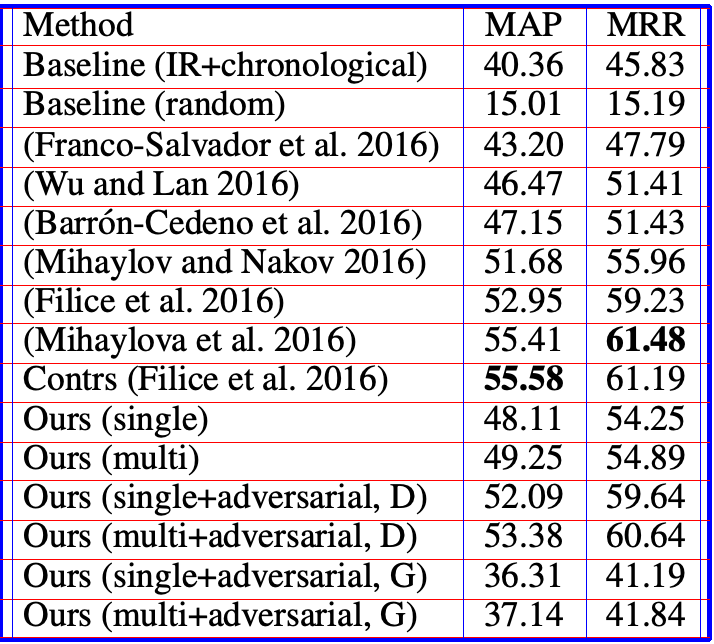
\includegraphics[width=\linewidth]{reconstructed_7.png}
		\end{minipage}
	\caption{The original table and the reconstructed table (4)}
	\label{fig6.8}
\end{figure}



\footnotetext[1]{\url{https://github.com/HazyResearch/pdftotree}}
\footnotetext[2]{Yang, Xiao, et al. "Adversarial training for community question answer selection based on multi-scale matching." Proceedings of the AAAI Conference on Artificial Intelligence. Vol. 33. No. 01. 2019.}

\section{Answers to Questions}

\begin{enumerate}
	\item \textbf{Q}: How to automatically locate the tables in a PDF?
	
	\textbf{A}: The table is very structured data. Therefore, we propose the following pipeline to automatically locate the tables in a PDF.
	\begin{enumerate}
		\item Parse each page from PDF and get the coordinates of characters and text lines for text detection;
		\item Preprocess the texts to remove all the blank spaces and special characters;
		\item Perform K-means clustring technique, and store the IDs and centroids of the clusters.
		\item Find the appropriate clusters, that is different from simple text cluster, then the cluster area should be a table.
		\item Check all clusters and then we can automatically locate all the tables in a PDF.
	\end{enumerate}

	In contemperary papers, tables all have a header, which should have be the destination of a hyper-link somewhere. Therefore, for this kind of papers, we just need to find all the hyper-links, and use the methods we proposed above to check whether it is a table.

	In our pipeline, we use a handy tool pdftotree\footnotemark[1] to automatically find the tables in the PDFs using pretrained machine learning models.

	\item \textbf{Q}: What do you think is the most difficult step to extract the table from the PDF? Why?
	
	\textbf{A}: Our pipeline only completes the prepositive works, such as extract tables from PDF file and perform table reconstruction by drawing framelines. The process is not very difficult, since we can use many handy tools to efficient parse a large batch of PDF files, extract tables according to bounding boxes coordinates, and draw framelines using digital image processing knowledges. \textbf{I think the most difficult step of the table reconstruction task is to further parse the reconstructed paper into structured data.} We know that the table may have various structures, such as merging several cells into one, \textit{etc}. Under such circumstances, our previous algorithm may divide the combined block into several blocks, and use several lines to represent a block. For example, our frameline-drawing algorithm may misidentify table structure as shown in Fig. \ref{fig6} in the next page.
	\footnotetext[1]{\url{https://github.com/HazyResearch/pdftotree}}
	\begin{figure}[htbp]
		\centering
			\begin{minipage}[t]{0.4\linewidth}
			\centering
			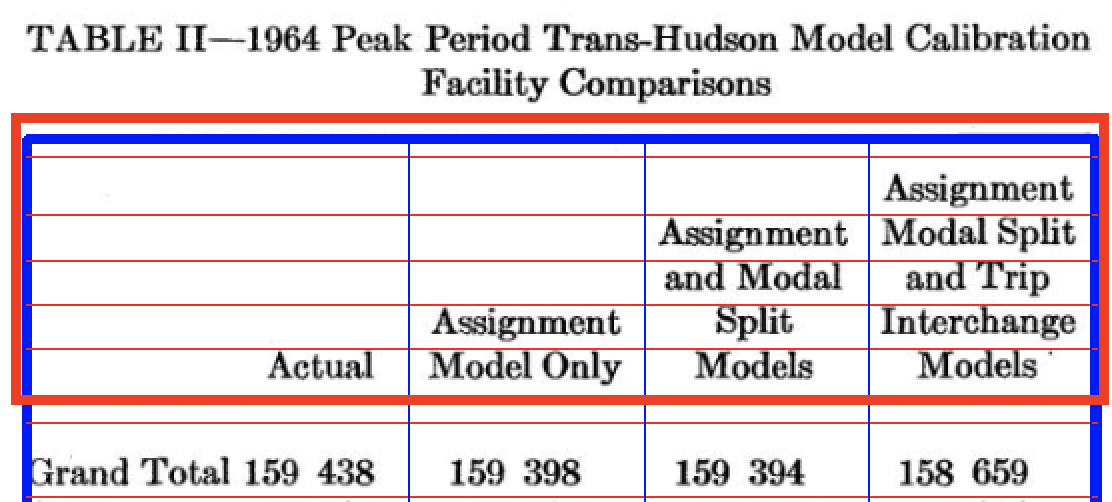
\includegraphics[width=\linewidth]{wrong1.png}
			\end{minipage}
			\begin{minipage}[t]{0.4\linewidth}
			\centering
			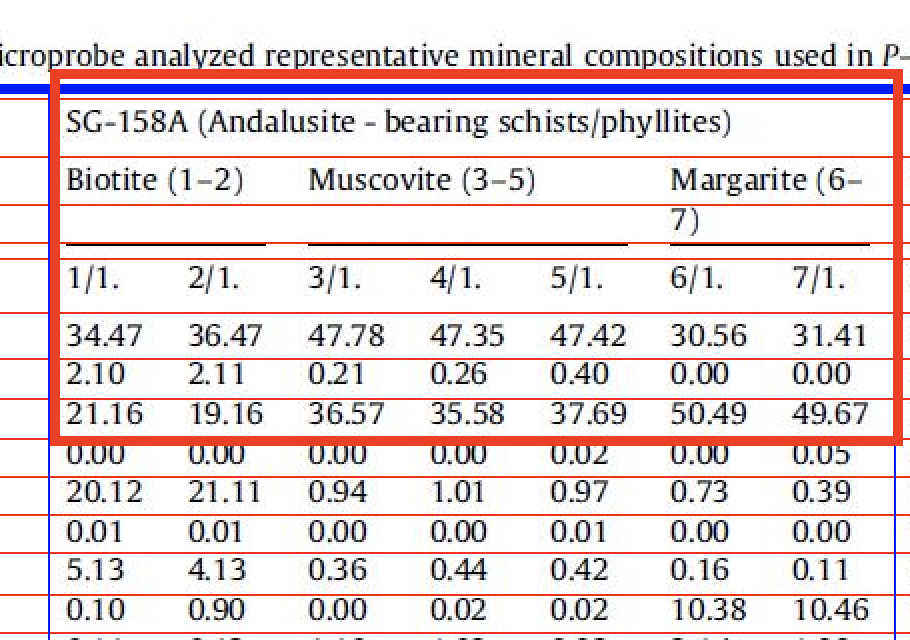
\includegraphics[width=\linewidth]{wrong2.png}
			\end{minipage}
		\caption{Examples of the misidentified situations (the red boxes)}
		\label{fig6}
	\end{figure}
	
	So how to identify the combined blocks and other special structure of the table, and then extract the information in the table to a structured data remains challenging. Therefore, I think this is the most difficult step to extract the table from the PDF.

	\item \textbf{(Bonus)} \textbf{Q}: How to accurately identify the header of the table, and use natural language processing (NLP) or other methods to understand the information in the table, and then extract the entities and relationships from table to construct a specific knowledge graph?
	
	\textbf{A}: 
	\textbf{Identify the header}: As mentioned above, \underline{for PDFs of the contemperary academic papers}, the table header must be hyper-linked by somewhere in the document. Therefore, we can simply check all the destination of all hyperlinks in the PDF file, then we can find all table headers. \underline{For old scanned documents of PDF format}, we may check the bold letters to find the word such as ``Table'' and ``Tab'' to find the tables. Actually, I think for those kind of documents, it is more like a computer vision task to recognize table headers from a given image. I think the classic computer vision network like ResNets\footnotemark[1] can have a great performance on detecting task like this.

	\footnotetext[1]{He, Kaiming, et al. "Deep residual learning for image recognition." Proceedings of the IEEE conference on computer vision and pattern recognition. 2016.}

	\textbf{Extract information in the table}: We can use OCR to extract texts in the pictures. According to our discussion in problem 2, the main challenge is how to get a structured table based on these informations. I would like to regard the task as a \textbf{image segmentation} task in computer vision field. We can regard each block in the table as a region and use image segmentation networks to learn how to divide the table into structured data.

	\textbf{Build a knowledge graph}: In this part, we may use the NLP models like Bert \footnotemark[2] to extract the connection between the row name and the column name. Then, we can regard the data as the label of the edge between row name and column name in the knowledge graph. Therefore, we can extract the embeddings from the tables to construct the knowledge graph.
	\footnotetext[2]{Devlin, Jacob, et al. "Bert: Pre-training of deep bidirectional transformers for language understanding." arXiv preprint arXiv:1810.04805 (2018).}
\end{enumerate}

\section{Conclusion}

In this lab, we explore the table reconstruction tasks of PDF files. I make clear explanations to the given code and modify the code a bit to satisfy the task settings. We have shown our reconstruction results and they are quite satisfiable: they can detect the table boundary accurately and reconstruct the table using several horizontal and vertical lines. We also propose a handy pipeline to extract tables from PDF files, and reconstruct it by drawing framelines.

We also explore further in the questions of how to extract information from the PDF file. We have proposed three ideas concerning three aspects:
\begin{itemize}
	\item Take the ``identify the header'' task as a computer vision task and use models like ResNets\footnotemark[1] to identify the header efficiently and effectively in scanned PDF documents. Check the destinations of hyper-links to identify the headers in today's PDf documents.
	\item Take the ``Extract information in the table'' as an image segmentation task. Recognize the texts using OCR techniques and extract the precise structure of the table using image segmentation models. Therefore, we can extract more accurate information from the table. Actually, the pdftotree\footnotemark[4] tool we used is based on the same idea.
	\item Take ``Build a knowledge graph'' as an natural language processing task. Use models like Bert\footnotemark[2] to extract embeddings from row name and column name. Then, use the data as the label of the edge between row name and the column name in the knowledge graph. Finally, extract the information you want from the built knowledge graph.
\end{itemize}

In conclusion, I gain knowledges from this lab and I think the lab benifits me a lot.

The full implementation codes of the lab is available in my \href{https://github.com/Galaxies99/EE447-CourseData/tree/main/Labs/Lab4}{github repository}. For other questions about the lab, please feel free to send an e-mail\footnotemark[3] to me.
\footnotetext[4]{\url{https://github.com/HazyResearch/pdftotree}}
\footnotetext[3]{\url{mailto:galaxies@sjtu.edu.cn}}
%========================================================================
\end{document}
